\section{Teórico}

  \definicion{Topic:} Density-functional perturbation theory (DFPT): phonons.

  \definicion{Speaker:} Stefano BARONI (SISSA, Italy).

\subsection{Funciones respuesta}

  Las funciones respuestas tienen la siguiente forma general
    $$propiedad = \frac{\partial variable}{\partial fuerza}$$

  donde \emph{fuerza} refiere a la fuerza de algún campo externo (eléctrico, magnético, de fuerzas/tensiones, etcétera).

  Permiten conocer tanto propiedades macroscópicas como microscópicas. En el caso miscroscópcio, la perturbación externa tiene el tamaño adecuado para lo que se pretende determinar.

\subsection{Teorema de Hellmann-Feynman}

  El ingrediente principal dentro de la teoría de funciones respuestas es el teorema HF.

  Pensémoslo primero en términos del Hamiltoniano y la energía. Supongamos que partimos de
    $$H_{\lambda} \Psi_{\lambda} = E_{\lambda} \Psi_{\lambda}$$

  donde el Hamiltoniano depende de un conjunto de parámetros externos ${\lambda}$ (aunque generalmente es una colección, puede ser un parámetro único), los cuales NO constituyen variables dinámicas. Luego, el teorema establece que
    $$\frac{\partial}{\partial \lambda} E_{\lambda} = \frac{\partial}{\partial \lambda} \expval{H_{\lambda}}{\Psi_{\lambda}}$$

  ya que el autovalor siempre puede pensarse como el valor de expectación del Hamiltoniano sobre los autoestados. Aplicando la regla de la cadena, se llega a
    $$\frac{\partial}{\partial \lambda} \expval{H_{\lambda}}{\Psi_{\lambda}} =
    \bra{\sfrac{\partial}{\partial \lambda} \Psi_{\lambda}} H_{\lambda} \ket{\Psi_{\lambda}} +
    \bra{\Psi_{\lambda}} \sfrac{\partial}{\partial \lambda}  H_{\lambda} \ket{\Psi_{\lambda}} +
    \bra{\Psi_{\lambda}} H_{\lambda} \ket{\sfrac{\partial}{\partial \lambda} \Psi_{\lambda}}$$
    $$= \bra{\Psi_{\lambda}} \sfrac{\partial}{\partial \lambda}  H_{\lambda} \ket{\Psi_{\lambda}} +
    E_{\lambda} \bra{\sfrac{\partial}{\partial \lambda} \Psi_{\lambda}} \ket{\Psi_{\lambda}} +
    E_{\lambda} \bra{\Psi_{\lambda}} \ket{\sfrac{\partial}{\partial \lambda} \Psi_{\lambda}} =
    \bra{\Psi_{\lambda}} \sfrac{\partial}{\partial \lambda}  H_{\lambda} \ket{\Psi_{\lambda}} +
    E_{\lambda} \frac{\partial}{\partial \lambda} \braket{\Psi_{\lambda}}$$

  Como los autoestados se suponen normalizados, tenemos que $\braket{\Psi_{\lambda}} = 1$ y, por lo tanto, $\frac{\partial}{\partial \lambda} \braket{\Psi_{\lambda}} = 0$. Se concluye entonces que
    $$\frac{\partial}{\partial \lambda} E_{\lambda} =
    \bra{\Psi_{\lambda}} \sfrac{\partial}{\partial \lambda}  H_{\lambda} \ket{\Psi_{\lambda}}$$

  Que la derivada del autovalor sea independiente de la derivada de los autovectores no es trivial: puedo avergiuar la derivada del autovalor con solo derivar el operador (y tomarle la media)!

  El teorema de HF se puede generalizar: es aplicable siempre que el problema se pueda escribir en términos de algún principio variacional. Supongamos que tenemos una función $g$ en función de un parámetro externo $\lambda$, la cual es el mínimo de un funcional $G$ que depende de una variable interna $x$ y el parámetro externo $\lambda$.
    $$g(\lambda) = \min_{x} G[x, \lambda]$$

  \Obs{En el caso de la energía nos quedaría
    $$E_{\lambda} = \min_{\Psi : \braket{\Psi}=1} \expval{H_{\lambda}}{\Psi}$$}

  El mínimos se encuentre derivando e igualando a cero: como $G$ depende de $\lambda$, el mínimo también depende de $\lambda$.
    $$\frac{\partial}{\partial x} G \Big|_{x = x (\lambda)} = 0 \Rightarrow g(\lambda) = G[x (\lambda), \lambda]$$

  Luego
    $$\frac{\partial}{\partial \lambda} g (\lambda) = \frac{\partial}{\partial x} G \Big|_{x = x (\lambda)} \frac{\partial}{\partial \lambda} x (\lambda) + \frac{\partial}{\partial \lambda} G \Big|_{x = x (\lambda)}$$

  Como estamos en el mínimo, sabemos que $\sfrac{\partial}{\partial x} G \Big|_{x = x (\lambda)} = 0$, con lo cual
    $$\frac{\partial}{\partial \lambda} g (\lambda) = \frac{\partial}{\partial \lambda} G [x, \lambda] \Big|_{x = x (\lambda)}$$

\subsection{Susceptibilidades: derivadas de la energía}

  La definición de susceptibilidad $\chi_{BA}$ es la derivada de un operador $B$ con respecto a un parámetro $\alpha$ que marca la fuerza de la perturbación. Se tiene que $A$ es una perturbación física mientras que $B$ es un observable.
    $$\chi_{BA} = \frac{\partial}{\partial \alpha} \expval{B}$$

  Supongamos que tenemos un Hamiltoniano que depende de una CL de perturbaciones $v_i$ con una contribución (fuerza) $\lambda_i$.
    $$H = H_0 + \sum_i \lambda_i v_i$$

  Luego la energía del sistema será
    $$E [\lambda] = E_0 - \sum_i f_i \lambda_i + \frac{1}{2} \sum_{ij} h_{ij} \lambda_i \lambda_j + ... $$

  donde la fuerza generalizada es $f_i = - \sfrac{\partial E}{\partial \lambda_i}$. Las derivadas primeras permiten determinar la optimización estructural y estudiar la dinámica molecular, mientras que las derivadas segundas $h_{ij}$ son funciones respuesta.

  Usando la nomenclatura de la teoría perturbacional, tenemos que
    $$f_i = - \expval{v_i}{\Psi_0} = - \int v_i (\vec{r}) \rho_0 (\vec{r}) d \vec{r}$$
    $$h_{ij} =  \int v_i (\vec{r}) \rho_j^{'} (\vec{r}) d \vec{r} = \int v_j (\vec{r}) \rho_i^{'} (\vec{r}) d \vec{r}$$

\subsection{DFPT}

  El potencial externo $V_{\lambda}$ actuando sobre el sistema lo podemos expandir según
    $$V_{\lambda} (\vec{r}) = V_0 (\vec{r}) + \sum_i \lambda_i v_i (\vec{r})$$

  Considerando cómo DFT define la energía y usando el teorema de HF se llega a que
    $$\frac{\partial^2}{\partial \lambda_i \partial \lambda_j} E (\lambda) = \int \frac{\partial}{\partial \lambda_j} n_{\lambda} (\vec{r}) v_i (\vec{r}) d \vec{r}$$

  Esta derivada segunada es la base de DFPT. Entonces para calcular la segunda derivada, debemos calcular la respuesta de la densidad de carga. Como $n$ es la suma sobre las normas cuadráticas de los autoestados KS, la derivada es sencilla de expresar. Usualmente los autoestados son reales, así que se peude olvidar la conjugación. Sin embargo a veces son útiles los estados de Bloch y ahí sí juega lo complejo.

  En DFPT lo que se hace es plantear un ciclo SCF análogoal de DFT y linealizar los 3 pasos (Fig. \ref{fig:DFPT}). Luego, se resuelve este nuevo ciclo SCF.

  \begin{figure}[H]
      \centering
      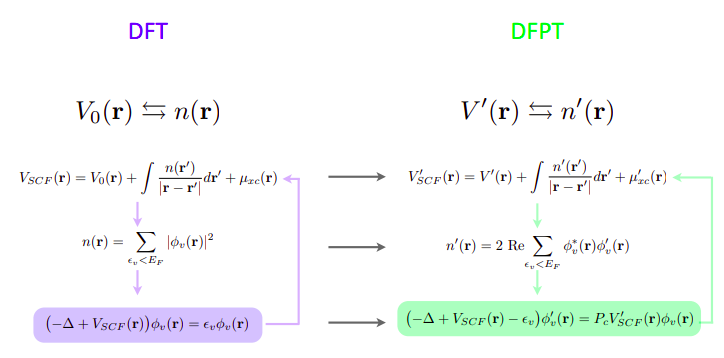
\includegraphics[scale = 0.6]{figs/D5/DFPT.png}
      \caption{DFT vs DFPT}
      \label{fig:DFPT}
  \end{figure}

\subsection{Simulación de vibraciones atómicas}

  Un cristal perfecto lo podemos describir como un potencial externo periódico (Fig. \ref{fig:red}). Queremos saber cuál es la respuesta del sistema respecto al desplazamiento individual de los átomos. A primer orden el potencial perturbativao es lineal en la amplitud de la distorsión atómica. Luego, para saber cómo depende la energía con la amplitud de la distorción, expandimos en Taylor y vemos que podemos pensarla directamente como curvatura o como derivadas primera de la fuerza. Esto se conoce como constante de fuerzas interatómicas (IFC) en el cotexto de la dinámica de redes.

  \begin{figure}[H]
      \centering
      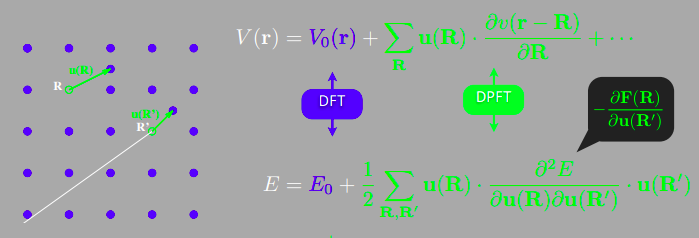
\includegraphics[scale = 0.6]{figs/D5/red.png}
      \caption{Dinámica de redes.}
      \label{fig:red}
  \end{figure}

  Ahora resolvemos la ecuación de autovalores para la matriz 3Nx3N de IFC (Fig. \ref{fig:vib}), la cual se conoce como matriz dinámica. Los autovalore son los cuadrados de las frecuencias vibracionales. Hay un factor $M$ que es la masa atómica, la cual puede incorporarse en el autovector.

    \begin{figure}[H]
      \centering
      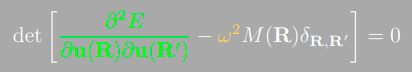
\includegraphics[scale = 0.6]{figs/D5/vibraciones.png}
      \caption{Problema de autovalores a resolver.}
      \label{fig:vib}
    \end{figure}

  Por la prueba de la derivada segunda, sabemos que el determinante tiene que ser positivo para asegurarnos que tenemos el mínimo. Esto se expresa con que los cuadrados de las frecuencias cuadradas tienen que ser positivas.

\subsection{Perturbaciones monocromáticas}

  Si queremos acomodar fonones de longitud de onda arbitraria, debemos hacer cálculos gigantes. Lo mejor es recurrir a la simetría: los fonones se clasifican en términos de sus números de onda. Los fonones de diferente longitud de onda no interactúan entre sí.

  Esto se refleja en DFPT al reescribir la longitud de onda en forma recíproca. Los orbitales no perturbados tiene vector de onda k definido (teorema de Bloch). Pero el fonon tiene vector de onda q. Entonces resulta que el número de onda general del resultado es k+q.

  Como el H es periódico, el KS orbital perturbado debe tener el mismo vector de onda (k+q): es un estado de Bloch. La densidad respuesta tiene el mismo número de onda que la perturbación. Lo mismo pasa con el potecial. Todo el cálculo puede mapearse entonces en calcular la parte periódica de la función de onda respuesta: la complejidad computacional del sistema yace en el número de electrones.

  \begin{figure}[H]
    \centering
    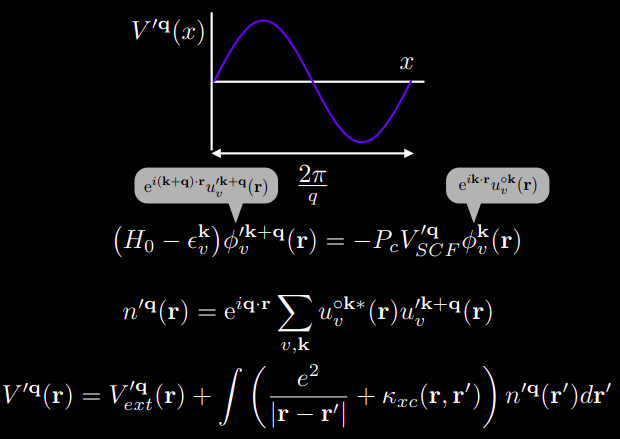
\includegraphics[scale = 0.5]{figs/D5/monocrom.png}
  \end{figure}

\subsection{Fonones en materiales polares}

  Generan un campo eléctrico macroscópico estos materiales. La energía depende de la distorción de red y del campo eléctrico. La parturbación tiene número de onda definido. El campo E es irrotacional en el espacio recíproco. En ausencia de cargas y corrientes: cuando la polarización del fonon es ortogonal a q, entonces la ecuación de Mawell se satisfce sólo cuando el campo es idénticamente nulo.

  Para los fonones transversales entonces la expresión es más sencilla. Ahora consideramos la otra ecuación de Mawell: se cumple sólo cuando D es nulo. Los fonones paralelos tienen otra expresión.

  Debemos tener una estimada de la carga efectiva y la constante electrica para calcular los fonones longitudinales.

  \begin{figure}[H]
    \centering
    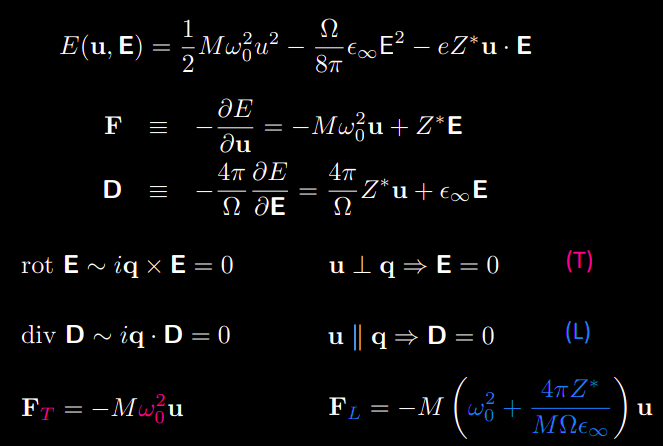
\includegraphics[scale = 0.5]{figs/D5/fonones_polares.png}
  \end{figure}

\subsection{Características principales DFPT}

  \begin{itemize}
    \item Calculo de funicones respuesta en términos de orbitales respuesta.
    \item Se resulven sistemas lineales sin calcular estados de conducción.
    \item Sólo se debe calcular la respuesta a la perturbación dada.
    \item También se pueden tratar perturbaciones no locales, no periódicas o campos eléctricos macroscópicos.
  \end{itemize}


\section{Q\&A}

  \definicion{Regarding acoustic phonons: how much is slightly different from zero? I mean when to consider it zero}

  It depends on the system and technicalities (xc functional, etc.). See point 7.2 here: https://www.quantum-espresso.org/resources/faq/phonons

  Let's say a few tens of $cm^{-1}$, more for lighter atoms (e.g. C), less for heavier atoms

  \definicion{does the enforcement of the acoustic sum rule shift every frequency at every q-point by the amount required by the first 3 modes at gamma? i.e., does it shift the whole phonon dispersion? or just the first 3 modes at gamma?}

  In principle, it should shift only the first 3 modes at gamma by a significant amount, all other modes by negligible amounts. If all modes change significantly after ASR, there is something not right.

  \definicion{Question: Is there a rule of thumb to choose the convergence criteria (conv\_thr) in scf.in input and (tr2\_ph) in ph.in . Which psuedopotential (norm-conserving or ultrsoft)  do you recommend to avoid having imaginary frequency.}

  For geometry optimizations I typically use conv\_thr = 1e-9 to 1e-10 (if the system converges that far), but instead of specifing conf\_thr=1e-9, I specify conf\_thr =1-e7 and upscale = 100.

  Note that conv\_thr is extensive and depends on the number of atoms, e.g. for 10x more atoms, multiply conv\_thr by 10.
  As for the tr\_ph: it is analogous to conv\_thr, but notice that it is a "square", hence conv\_thr =1e-8 would corresponds to tr2\_ph = 1e-16.

  Type of  pseudopotential have nothing to do with imaginary frequencies.

  \definicion{For phonon calculations to obtain the frequencies, how do I choose the q mesh? What do I follow to check for convergence?}

  You should in principle to check the convergence of the dispersion with respect to the size of the q-mesh. In order to do that, you can rerun the ph-q2r-matdyn chain of calculations for a different size of the mesh, which you specify in the input file of ph.x (nq1, nq2, nq3 variables). Then, you check how the dispersions look like and you compare each dispersion. As a rule of thumb, if the frequencies change by about or less than 10 cm-1 (few cm-1 is fine) the convergence of the interpolation is reasonable

\section{Hands-on}

  \definicion{Topic:} DFPT.

  \definicion{Speaker:} Andrea URRU (ETH, Switzerland), Iurii TIMROV (EPFL, Switzerland).

\subsection{Materiales no polares: Si}

  Vamos a calcular para Si las frecuencias fonónicas en el punto $\Gamma$ (example1a) y la dispersión fonónica (example1b).

\subsubsection{Punto $\Gamma$}

  Primero vamos a calcular los fonones en $\Gamma$. Dentro de la carpeta tenemos:
    \begin{itemize}
      \item $pw.Si.in \Rightarrow$ SCF del estado fundamental.
        \begin{verbatim}
          mpirun -np 2 pw.x < pw.Si.in > pw.Si.out
        \end{verbatim}
      \item $ph.Si.in \Rightarrow$ cálculo de fonones en $\Gamma$.
      \begin{verbatim}
        mpirun -np 2 ph.x < ph.Si.in > ph.Si.out
      \end{verbatim}
      \item $dynmat.Si.in \Rightarrow$ imposición de la ASR.
      \begin{verbatim}
          mpirun -np 2 dynmat.x < dynmat.Si.in > dynmat.Si.out
      \end{verbatim}
    \end{itemize}

  En el input de ph.x vemos que:
    \begin{itemize}
      \item Luego de la namelist \&inputph ponemos las coordenadas del vector de onda ($q=\sfrac{2\pi}{a}$) donde queremos calcular los fonones.
      \item El ubral para la SCF es varios órdenes menor: como necesitamos derivadas segundas, tenemos que ir más abajo.
      \item Le indicamos dónde queremos que ponga la matriz dinámica.
    \end{itemize}

  Como en la Si tenemos dos átomos en la celda unidad, tendremos 6 modos fonónicos. Se resuelven de a tres por simetría. Cuando ddv\_scf\^2 es menor que el umbral que le dimos en el input, se considera alcanzada la convergencia. Luego de la convergencia se encuentran las frecuencias.

  En el ph.Si.out encontramos lo siguiente:
  \begin{figure}[H]
    \centering
    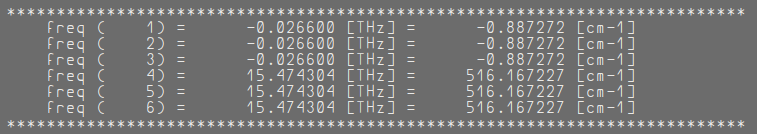
\includegraphics[scale = 0.6]{figs/D5/Si_ph.png}
  \end{figure}

  De los 6 modos que tenemos, 3 son acústicos y 3 son ópticos. Siempre se espera que haya 3 modos acústicos y el resto son modos ópticos.

  Vemos que los 3 modos acústicos son negativos, lo cual indica que el cuadrado de la freq es negativa: se tienen frecuencias imaginarias. Esto sería un signo de inestabilidad. Sin embargo, se pede ver que en este caso justo corresponde a ruido numérico, porque son negativas, pero muy cercanas a cero. Más allá de eso, estamos calculando en $\Gamma$ y ahí los modos acústicos deberían ser exactamente nulos debido a que son traslaciones rígidas del cristal. Por la invariancia traslacional, la energía del sistema es invariante y de allí que la frecuencia debe ser nula.

  Los errores numéricos provocan que las IFC no satisfagan de manera estricta la ASR (Acoustic Sum Rule).

  Todo este problema se soluciona con dynmat.x: esto impone la ASR. Luego, en el dynmat.out vemos las frecuencias de la matriz dinámica corregidas: ahora los modos acústicos sí son cero.

  \begin{figure}[H]
    \centering
    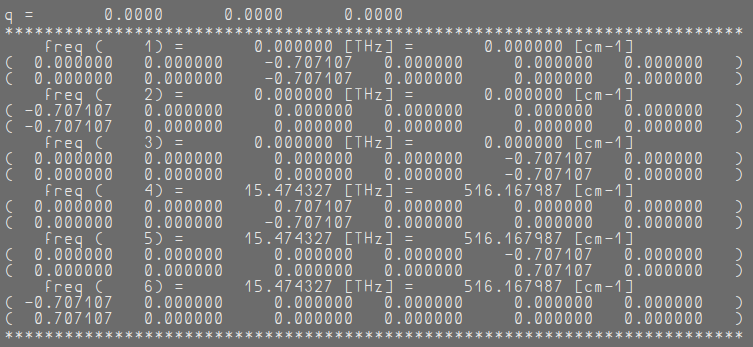
\includegraphics[scale = 0.6]{figs/D5/ASR.png}
  \end{figure}

\subsubsection{Dispersión fonónica}

  Ahora vamos a calcular la dispersión fonónica de Si. Para esto podríamos obtener las curvas corriendo punto a punto. Esto sería infinitamente largo. La alternativa razonable es hacer una interpolación de Fourier:
    \begin{enumerate}
      \item Calcular las matrices dinámicas sobre el espacio recíproca para una cantidad pequeña de puntos q.
      \item Hacemos la antitransformada de Fourier a partir de la información que tenemos con esta mesh poco densa. Esto nos permite conocer la IFC sobre todo el espacio real (claro que a mayor densidad de la mesh, mejor es este conocimiento, pero no importa: sabemos mucho igual).
      \item Luego hacemos la transformada de Fourier para volver al espacio recíproco, pero ahora podemos elegir cualquier vector q, sin relación alguna con los del comienzo. Los que vamos a usar son aquellos que se ubican  sobre los caminos de alta simetría.
    \end{enumerate}

    \begin{figure}[H]
      \centering
      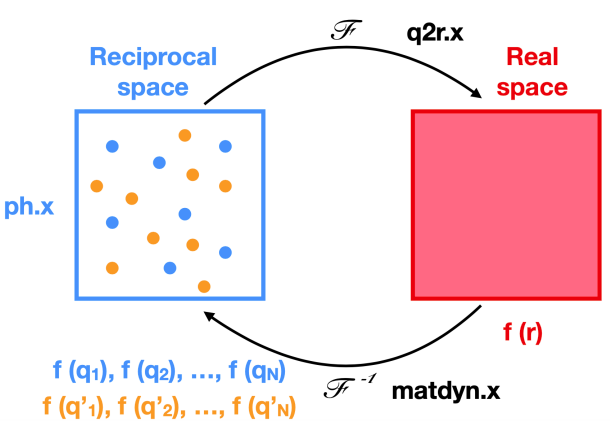
\includegraphics[scale = 0.6]{figs/D5/Fourier.png}
    \end{figure}

  \Obs{Se llama de Fourier porque la interpolación necesita ir y volver entre espacios duales. Tranquilamente podemos tener 10 puntos de inicio y después pedirle 400.}

  Los pasos a seguir son:
    \begin{enumerate}
      \item Concoer el estado fundamental.
        \begin{verbatim}
          mpirun -np 2 pw.x < pw.Si.in > pw.Si.out
        \end{verbatim}
      \item Hacer el cálculo de fonones sobre una mesh uniforme de puntos q (4x4x4 da 8 puntos no equivalentes). (OJO: cambia la forma en la que se pide mesh uniforme en el input respectoa pedirle q puntuales)
      \begin{verbatim}
        mpirun -np 2 ph.x < ph.Si.in > ph.Si.out
      \end{verbatim}
      \item Hacer la antitransformada de las IFC.
      \begin{verbatim}
        mpirun -np 2 q2r.x < q2r.Si.in > q2r.Si.out
      \end{verbatim}
      \item Hacer la transformada para calcular las frecuencias genéricas a partir de las IFC (la vuelta la hacemos con 396 puntos).
      \begin{verbatim}
        mpirun -np 2 matdyn.x < matdyn.Si.in > matdyn.Si.out
      \end{verbatim}
      \item Plotear. El plotband.x es puramente secuencial.
      \begin{verbatim}
        plotband.x < plotband.Si.in > plotband.Si.out
        gnuplot plot_dispersion.gp
        atril phonon_dispersion.eps
      \end{verbatim}
    \end{enumerate}

  ¿Cómo saber que estamos usando una grilla \emph{gruesa} lo \emph{suficientemente fina}? Hacer pruebas. Corroborar visualmente si hay cambios muy graves. Comparar 2x2x2 4x4x4 6x6x6 8x8x8. Hacer plotban para cada grilla.

  Otra manera es hacer un cálculo directo. Como es una interpolación, se puede hacer una single q vector calculation. Calcular algunitos y ver que caigan sobre la curva generada con la mesh dada.

  Cualquiera de los dos caminos va a andar bien.
  \begin{figure}[H]
    \centering
    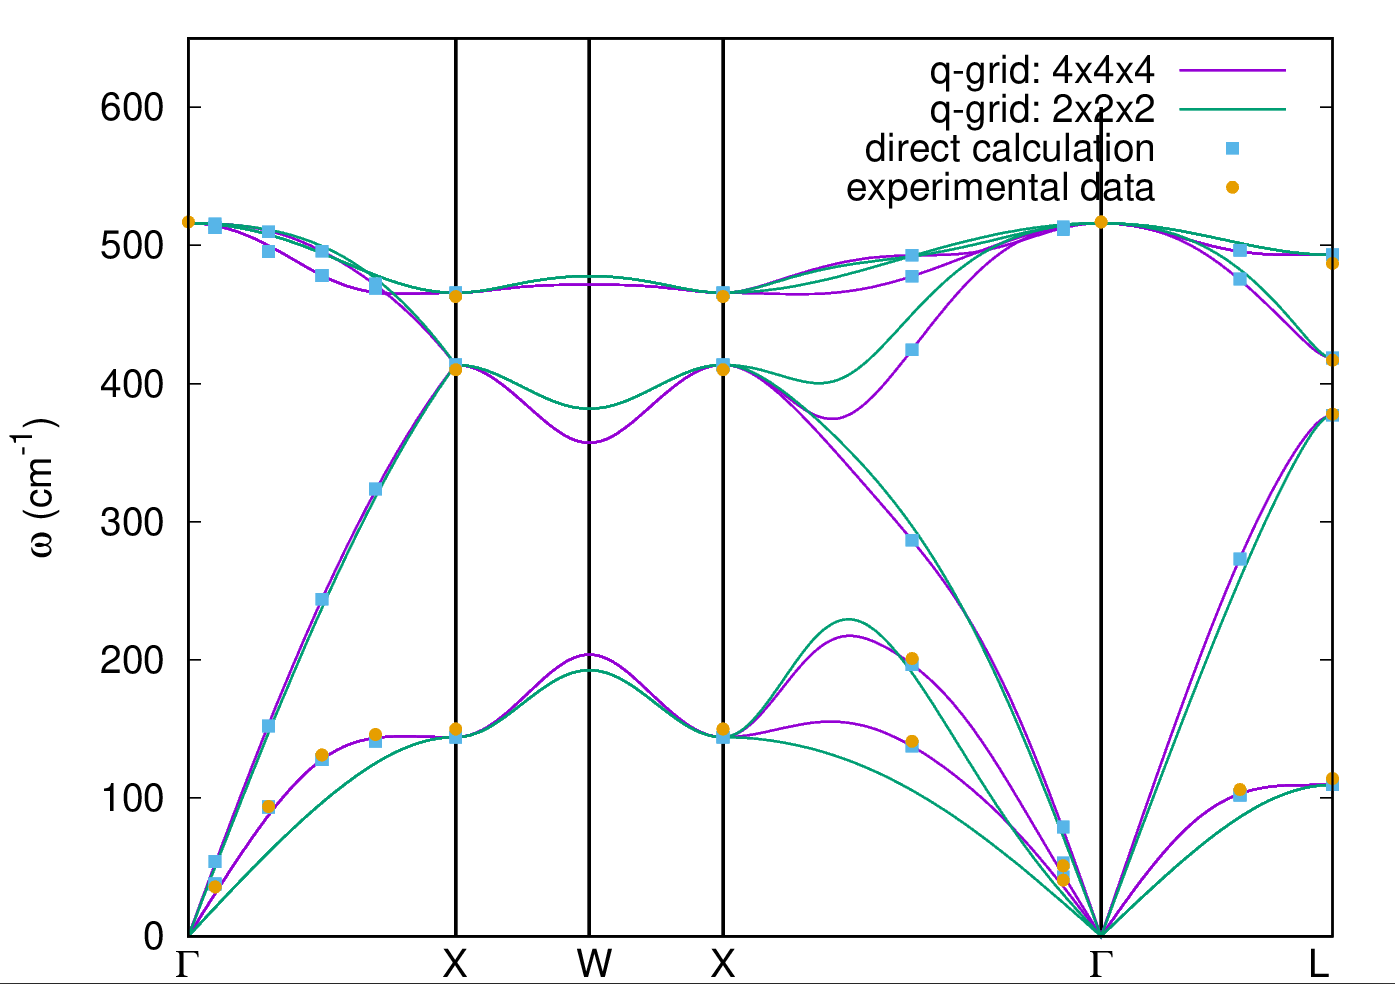
\includegraphics[scale = 0.35]{figs/D5/Si_disp.png}
  \end{figure}

\subsection{Materiales polares: AlAs}

  Vamos a calcular para AlAs las frecuencias fonónicas en el punto $\Gamma$ (example2a) y la dispersión fonónica (example2b).

\subsubsection{Punto $\Gamma$}

  Primero vamos a calcular los fonones en $\Gamma$. Dentro de la carpeta tenemos:
    \begin{itemize}
      \item $pw.AlAs.in \Rightarrow$ SCF del estado fundamental.
        \begin{verbatim}
          mpirun -np 2 pw.x < pw.AlAs.in > pw.Si.out
        \end{verbatim}
      \item $ph.AlAs.in \Rightarrow$ cálculo de fonones en $\Gamma$.
      \begin{verbatim}
        mpirun -np 2 ph.x < ph.Si.in > ph.Si.out
      \end{verbatim}
      \item $dynmat.AlAs.in \Rightarrow$ imposición de la ASR junto a la adición de la separación no analítica LO-TO (Longitudinal Optical - Transversed Optical).
      \begin{verbatim}
          mpirun -np 2 dynmat.x < dynmat.AlAs.in > dynmat.AlAs.out
      \end{verbatim}
    \end{itemize}

  Ahora tenemos un semiconductor polar por lo que aparece una contribución no analítica en $q=0$. En el input del ph.x tengo que poner $epsil = .true.$ para que haga el cálculo con el campo elécctrico que hace falta y así determinar las cargas efectivas y el tensor dieléctrico.

  El programa ph.x sólo calcula la parte analítica de la matriz dinámica, \emph{i.e.} todavía no incorporamos la corrección para $q=0$. Luego, no aparece aún la separación LO-TO: las 3 frecuencias ópticas están degeneradas dada la simetría del sistema. Vemos además que los modos acústicos no son idénticamente nulos como debería ser.

  \begin{figure}[H]
      \centering
      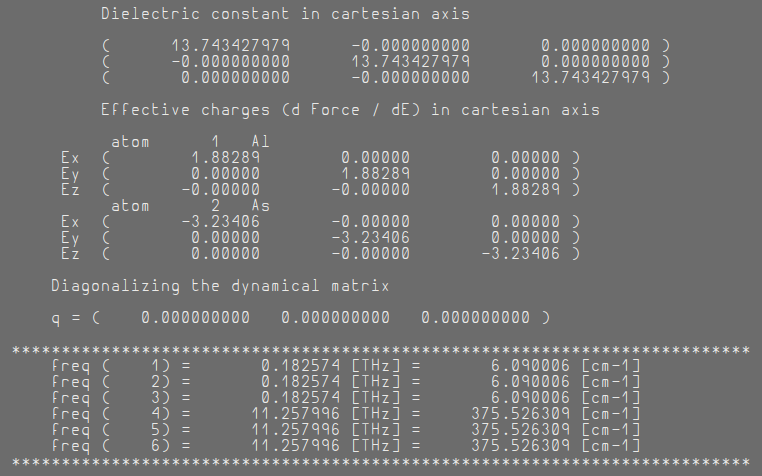
\includegraphics[scale = 0.6]{figs/D5/AlAs_pre.png}
  \end{figure}

  Como vimos en el ejemplo anterior, cada vez que queremos incluir una correción en la matriz dinámica, debemos ejecutar dynmat.x: ahora en el input incluimos el vector $q$ que determina al dirección  de aproximacion al punto $\Gamma$. En este caso nos estamos acercando a lo largo del semieje x positivo.
    \begin{verbatim}
      q(1) = 1.0, q(2) = 0.0, q(3) = 0.0
    \end{verbatim}

  Al incluir el término no analítico se levanta la degeneración de los modos ópticos: tenemos el LO-TO spliting.
    \begin{figure}[H]
        \centering
        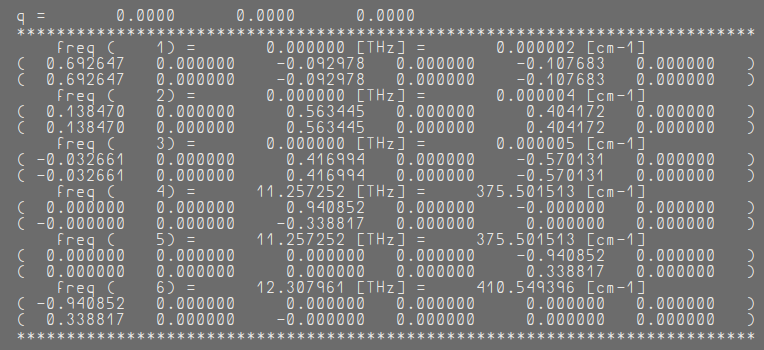
\includegraphics[scale = 0.6]{figs/D5/AlAs_post.png}
    \end{figure}

\subsubsection{Dispersión fonónica}

  Si calculamos la dispersión fonónica completa de AlAs, podremos ver el splitting LO-TO en las proximidades de $\Gamma$.

  \Obs{Los inputs tienen ariables faltates. Aquello que falta está con un comentario al lado.}

  Vemos que en torno al $\Gamma$ ocurre el LO-TO splitting.

    \begin{figure}[H]
        \centering
        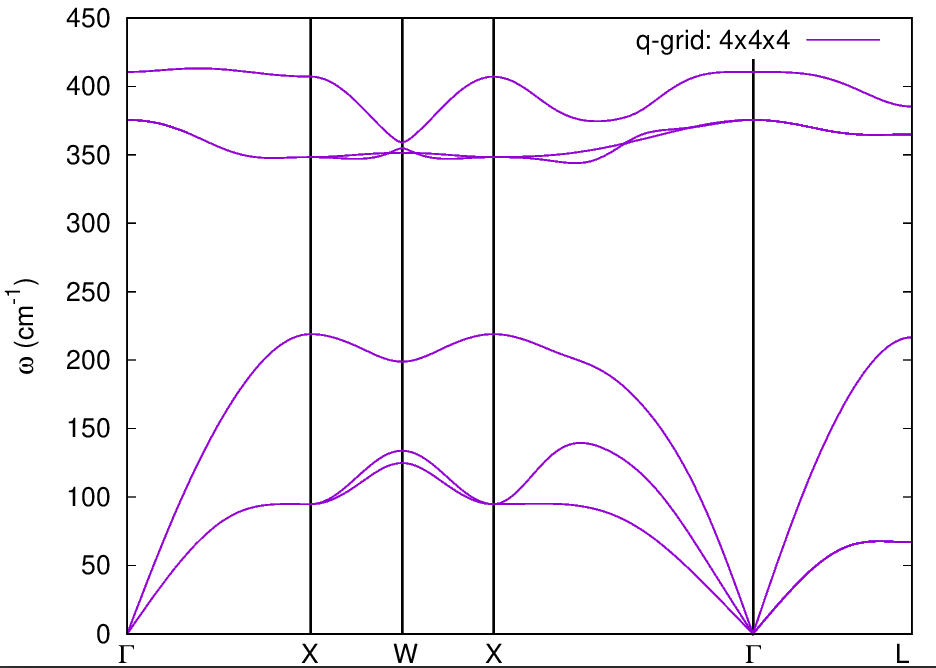
\includegraphics[scale = 0.4]{figs/D5/AlAs_disp.png}
    \end{figure}

\subsection{Materiales 2D: BN hexagonal}

  Vamos a calcular la dispersión fonónica para el caso de BN hexagonal. Los pasos a realizar son los mismos que antes. Vemos que en el input de pw.x está $assume\_isolated='2D'$ lo cual permite eliminar la interacción dipolo dipolo entre las capaz del material si es que existieran. Además está $loto\_2d=.true.$ tanto para q2r.x como para matdyn.x para que no desaparezca, si existe, la separación LO-TO.

  \Obs{No corre en los 20 CPU, así que hay que poner NPROC=8 antes del mpirun. Una alternativa al $assume\_isolated$ es ir aumentando el vacío entre láminas y vamos viendo que el spliting va disminuyendo de ancho. Esto no es muy sensato computacionalmente ya que el ancho de la separación tiende a cero de manera lineal en una log-log.}

  Vemos algunas catacterísticas propias de materiales 2D:
    \begin{itemize}
      \item El tercer modo acústico no crece lineal sino cuadrático al alejarse de $\Gamma$ (flexural mode).
      \item No hay LO-TO splitting en $\Gamma$ a pesar de ser un material polar.
    \end{itemize}

    \begin{figure}[H]
        \centering
        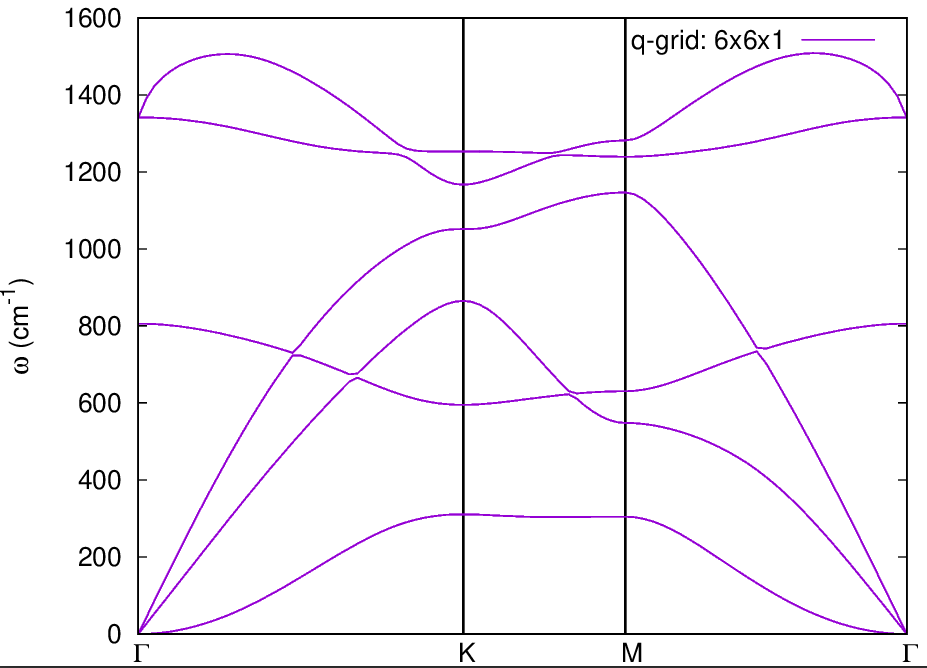
\includegraphics[scale = 0.4]{figs/D5/BN_disp.png}
    \end{figure}
